%!TEX root = ../AliStrangeJets.tex

\section{Analysis}%
\label{sec:Analysis}

\subsection{Charged jet reconstruction}%
\label{sec:JetRec}

In this analysis, the FastJet package~\cite{Cacciari:2011ma} is used to find jets using charged particles with the so-called \akT algorithm.
The \akT algorithm is a commonly known jet finding algorithm that starts the clustering with the highest momentum particles, in contrast to the $\kT$ algorithm, which does the opposite.
The introduction of the algorithm can be found in \cite{Cacciari:2008gp}.
Charged particles, which are used as the jet reconstruction inputs, are reconstructed using ITS and TPC information.
The charged particle are selected in $\abs{\eta_{\rm trk}} < 0.9$ ($\TPC$ acceptance) and $\pT> 0.15$~\GeVc.
The jet resolution parameter is $R = 0.4$ and the reconstructed jet clusters are selected in $\abs{\eta_{\rm jet}} < 0.35$.
A cut on charged-particle jet $\pT$ ($\pTj^{\rm ch}$) is applied as $\pTj^{\rm ch} > 10$~\GeVc.

Besides the hard parton-parton interactions in the collisions, there is also the soft contribution summarizing everything that did not correlate with the hard collisions.
The background density is around $1$~\GeVc~rad$^{-1}$ and is not subtracted on jet-by-jet basis in \pp collisions.
In \pPb collisions, the reconstructed jet is further corrected for contributions form the underlying event to the jet momentum as
\begin{equation}
\pTj = \pTjch - \rhobkg\cdot\Ajet
\label{eq:DeltaPt}
\end{equation}
where the $\pTj^{\rm rec}$ is the reconstructed jet $\pT$, $\Ajet$ is the jet area and $\rhobkg$ is the event-by-event background density~\cite{Cacciari:2007fd}.
The $\Ajet$ is calculated using the Fastjet algorithm with the ghost area $0.005$~\cite{Cacciari:2008gn}.
A method that is suitable for combinatory jet background density (\rhobkg) estimation for sparse systems circumvents circumventing the problems arising from using the ghost jets is introduced in \cite{Chatrchyan:2012tt}.
The basic idea is to neglect the ghosts and instead account for the empty areas by introducing a factor correcting the background density for it.
It can be implemented by the following approach
\begin{equation}
\rhobkg = C\cdot{\rm median}\{\frac{p_{\rm T,i}}{A_{i}}\},~{\rm with}~C = \frac{\sum_{j} A_{j}}{A_\mathrm{acc}}
\label{eq:RhoCMS}
\end{equation}
Technically, the occupancy correction factor $C$ is calculated as the ratio of $\kT$ jet clusters built by pure ghosts overall $\kT$ jet clusters.
This method has the advantage that it uses the median and takes empty areas into account and that it does not have conceptual problems like other methods.
This method can be further refined for the specific use case of \pPb collisions.
It can be shown that the exclusion of the first two $\kT$ jets from Eq.~(\ref{eq:RhoCMS}) is enhancing the background quality.

\subsection{Strange particles reconstruction}%
\label{sec:ParRec}

The strange particles \kzero, \lmb, \almb, \Xis and \Oms are reconstructed at mid-rapidity ($\abs{\eta} < 0.75$) with their specific weak decay topology.
The following decay channels are studied~\cite{PhysRevD.98.030001}.
$$
\begin{aligned}
\kzero      & \to \pip + \pim               & B.R. & = (69.20 \pm 0.05) \% \\
\lmb (\almb) & \to p(\pbar) + \pim (\pip)    & B.R. & = (63.9  \pm 0.5)  \% \\
\X (\Ix)    & \to \lmb (\almb) + \pim (\pip) & B.R. & = (99.887 \pm 0.035) \% \\
\Om (\Mo)   & \to \lmb (\almb) + \kam (\kap) & B.R. & = (67.8  \pm 0.7)  \% \\
\end{aligned}
$$
The proton, pion, and Kaon tracks (daughter tracks) are identified in the TPC via their measured energy deposition~\cite{Abelev:2014ffa}.
The identification methods for the \Vzero (\kzero and \lmb (\almb) which decay into two oppositely charged daughter particles) and cascade (\Xis and \Oms which decay into a charged meson (bachelor) plus a \Vzero decaying particle, giving the two-step process) candidates follow those presented in earlier ALICE publications~\cite{Aamodt:2011zza, Abelev:2012jp, Acharya:2018orn, Abelev:2013haa, Acharya:2020uxl, Acharya:2019kyh}.
In addition, to remove the contribution from pileup collisions outside the trigger proton bunch (out-of-bunch pileup), it is requested that at least one of the tracks from the decay products of the (multi-)strange hadron understudy is matched in either the ITS or TOF detector.
The selections used in this paper are summarized in Tab.~\ref{tab:V0Cut}, \ref{tab:CascadeCut}
\begin{table}[!ht]
	\begin{center}
		\caption{\Vzeros (\kzero, \lmb and \almb) candidate selection criteria of topological variable, daughter track and candidate.
			The DCA stands for ``Distance of Closest Approach'', PV represents the ``Primary collision Vertex'' and CPA is the ``Cosine Pointing Angle between the momentum vector of the reconstructed \Vzero and the displacement vector between the decay and primary vertices''.}
		\label{tab:V0Cut}
		\begin{tabularx}{\textwidth}{@{} lCC @{}}
			\toprule
			\textbf{Topological variable} & \textbf{\pp} & \textbf{\pPb} \\
			\midrule
			$\Vzero$ transverse decay radius      & $> 0.5$~cm   & $> 0.5$~cm \\
			DCA of positive / negative track to PV & $> 0.06$~cm  & $> 0.06$~cm \\
			DCA between $\Vzero$ daughter tracks  & $< 1.0\sigma$ & $< 1\sigma$ \\
			CPA of $\Vzero$ & $> 0.97$ ($\kzero$); $>0.995$ ($\lmb$) & $> 0.97$($\kzero$); $>0.995$ ($\lmb$) \\
			\midrule
			\textbf{Track selection} \\
			\midrule
			Daughter track pseudo-rapidity interval &$|\eta| < 0.8$ & $\abs{\eta} < 0.8$      \\
			Daughter track $N_{\rm crossed~rows}$                   & $\geq 70$  & $\geq$ 70 \\
			Daughter Track $N_{\rm crossed~rows}/N_{\rm findable}$  & $\geq 0.8$ & $\geq$ 0.8 \\
			TPC $\dEdx$ & $< 5\sigma$ & $< 5\sigma$ \\
			\midrule
			\textbf{Candidate selection} \\
			\midrule
			Pseudo-rapidity interval & $|\eta| < 0.75$ & $|\eta| < 0.75$ \\
			Proper lifetime($mL/p$)  & $< 20$~cm ($\kzero$), $< 30$~cm ($\lmb$) & $<20$~cm ($\kzero$), $< 30$~cm($\lmb$) \\
			Competing mass for \kzero & $> 0.005$~\GeVmass & $> 0.005$~\GeVmass \\
			Competing mass for \lmb  & $> 0.010$~\GeVmass & $> 0.010$~\GeVmass \\
			\bottomrule
		\end{tabularx}
	\end{center}
\end{table}

\begin{table}[!ht]
	\begin{center}
		\caption{\Xis and \Oms candidate selection criteria of topological variable, daughter track and candidate.}
		\label{tab:CascadeCut}
		\begin{tabularx}{\textwidth}{@{} lCC @{}}
			\toprule
			\textbf{Topological variable} & \textbf{\pp} & \textbf{\pPb} \\
			\midrule
			Cascade transverse decay radius & $> 0.8(0.6)$~cm & $> 0.6$~cm \\
			\Vzero transverse decay radius & $> 1.4$~cm     & $> 1.2$~cm \\
			DCA (bachelor to PV)           & $> 0.05$~cm    & $> 0.04$~cm \\
			DCA (\Vzero to PV)             & $> 0.07$~cm    & $> 0.06$~cm \\
			DCA (positive / negative track to PV) & $> 0.04(0.03)$~cm & $> 0.03$~cm  \\
			DCA between \Vzero daughter tracks & $< 1.6\sigma$     & $< 1.5\sigma$ \\
			DCA (bachelor to \Vzero) & $< 1.6(1.0)$~cm & $< 1.3$~cm \\
			CPA of Cascade          & $> 0.97$       & $> 0.97$  \\
			CPA of \Vzero           & $> 0.97$       & $> 0.97$  \\
			\Vzero invariant mass window & $\pm 0.006$~\GeVmass & $\pm 0.008$~\GeVmass \\
			\midrule
			\textbf{Track selection} \\
			\midrule
			Daughter track pseudo-rapidity interval & $|\eta| < 0.8$ & $|\eta| < 0.8$ \\
			Daughter track $N_{\rm crossed~rows}$  & $\geq 70$      & $\geq$ 70 \\
			Daughter Track $N_{\rm crossed~rows}/N_{\rm findable}$ &$\geq 0.8$ &$\geq$ 0.8 \\
			TPC $\dEdx$ & $< 5\sigma$ & $< 4\sigma$ \\
			\midrule
			\textbf{Candidate selection} \\
			\midrule
			Pseudo-rapidity interval & $|\eta| < 0.75$ &$|\eta| < 0.75$ \\
			Proper lifetime ($mL/p$) & & $< 3 \times c\tau$ \\
			Competing mass          & $8$~\MeVmass & $8$~\MeVmass \\
			\bottomrule
		\end{tabularx}
	\end{center}
\end{table}
The signal extraction is performed as a function of $\pT$.
In each $\pT$ interval, an invariant mass histogram is produced and filled with the corresponding counts.
Then a Gaussian function is used to fit the peak, and a liner function is used to fit the combinatory background.
This allows for the extraction of the mean ($\mu$) and width ($\sigma$) of the peak.
A ``peak'' region is defined within $\pm 6\sigma$ for $\Vzeros$ and $\pm 3\sigma$ ($\pm 4\sigma$) for cascades in \pp (and \pPb) with respect to $\mu$ for each $\pT$ bin.
The ``background'' regions are defined on both sides of that central region.
The $\pT$-differential yields of (multi-)strange particles are extracted by fitting the background with a linear function extrapolated under the signal region.
Examples of the invariant mass peaks for all particles are shown in Fig.~\ref{fig:InvM}.
\begin{figure}[!ht]
	\begin{center}
		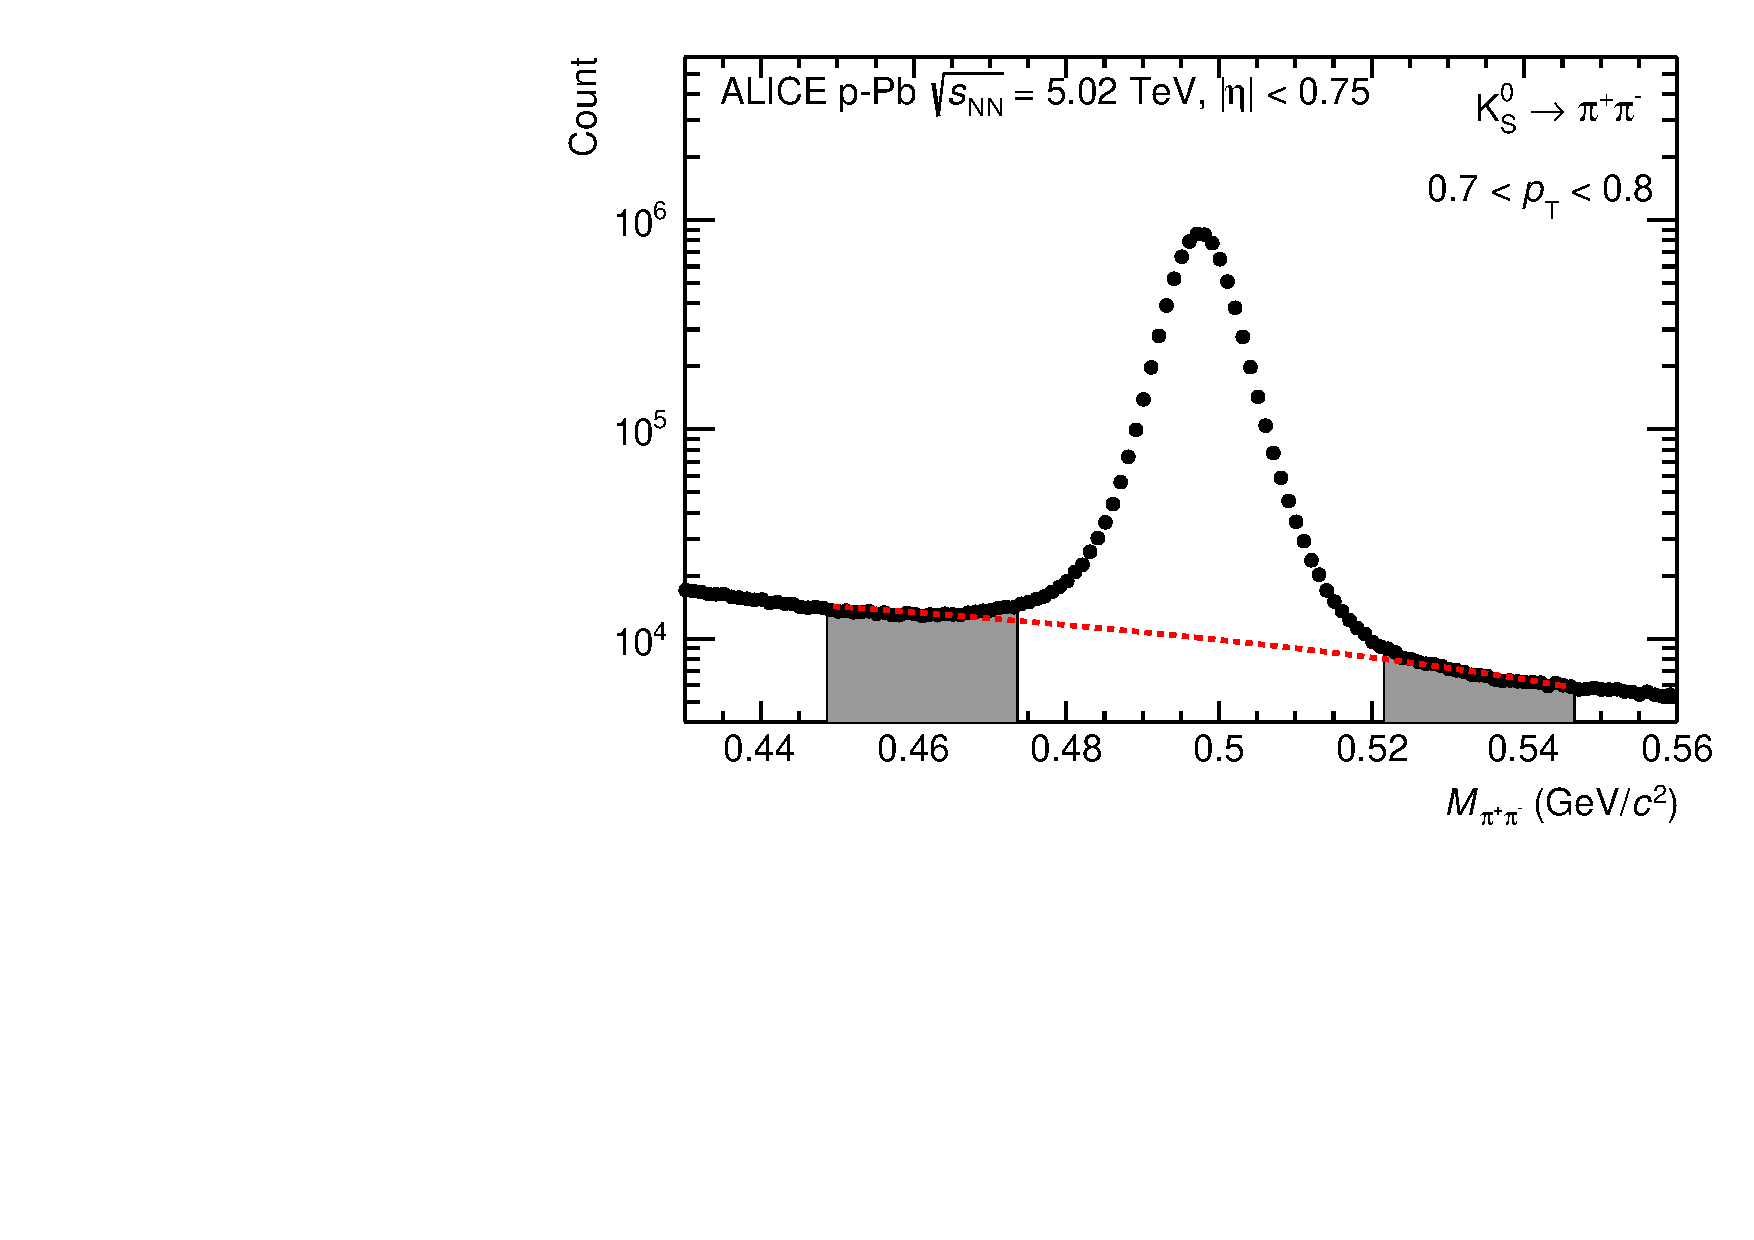
\includegraphics[width=.4\textwidth]{cf01_1}
		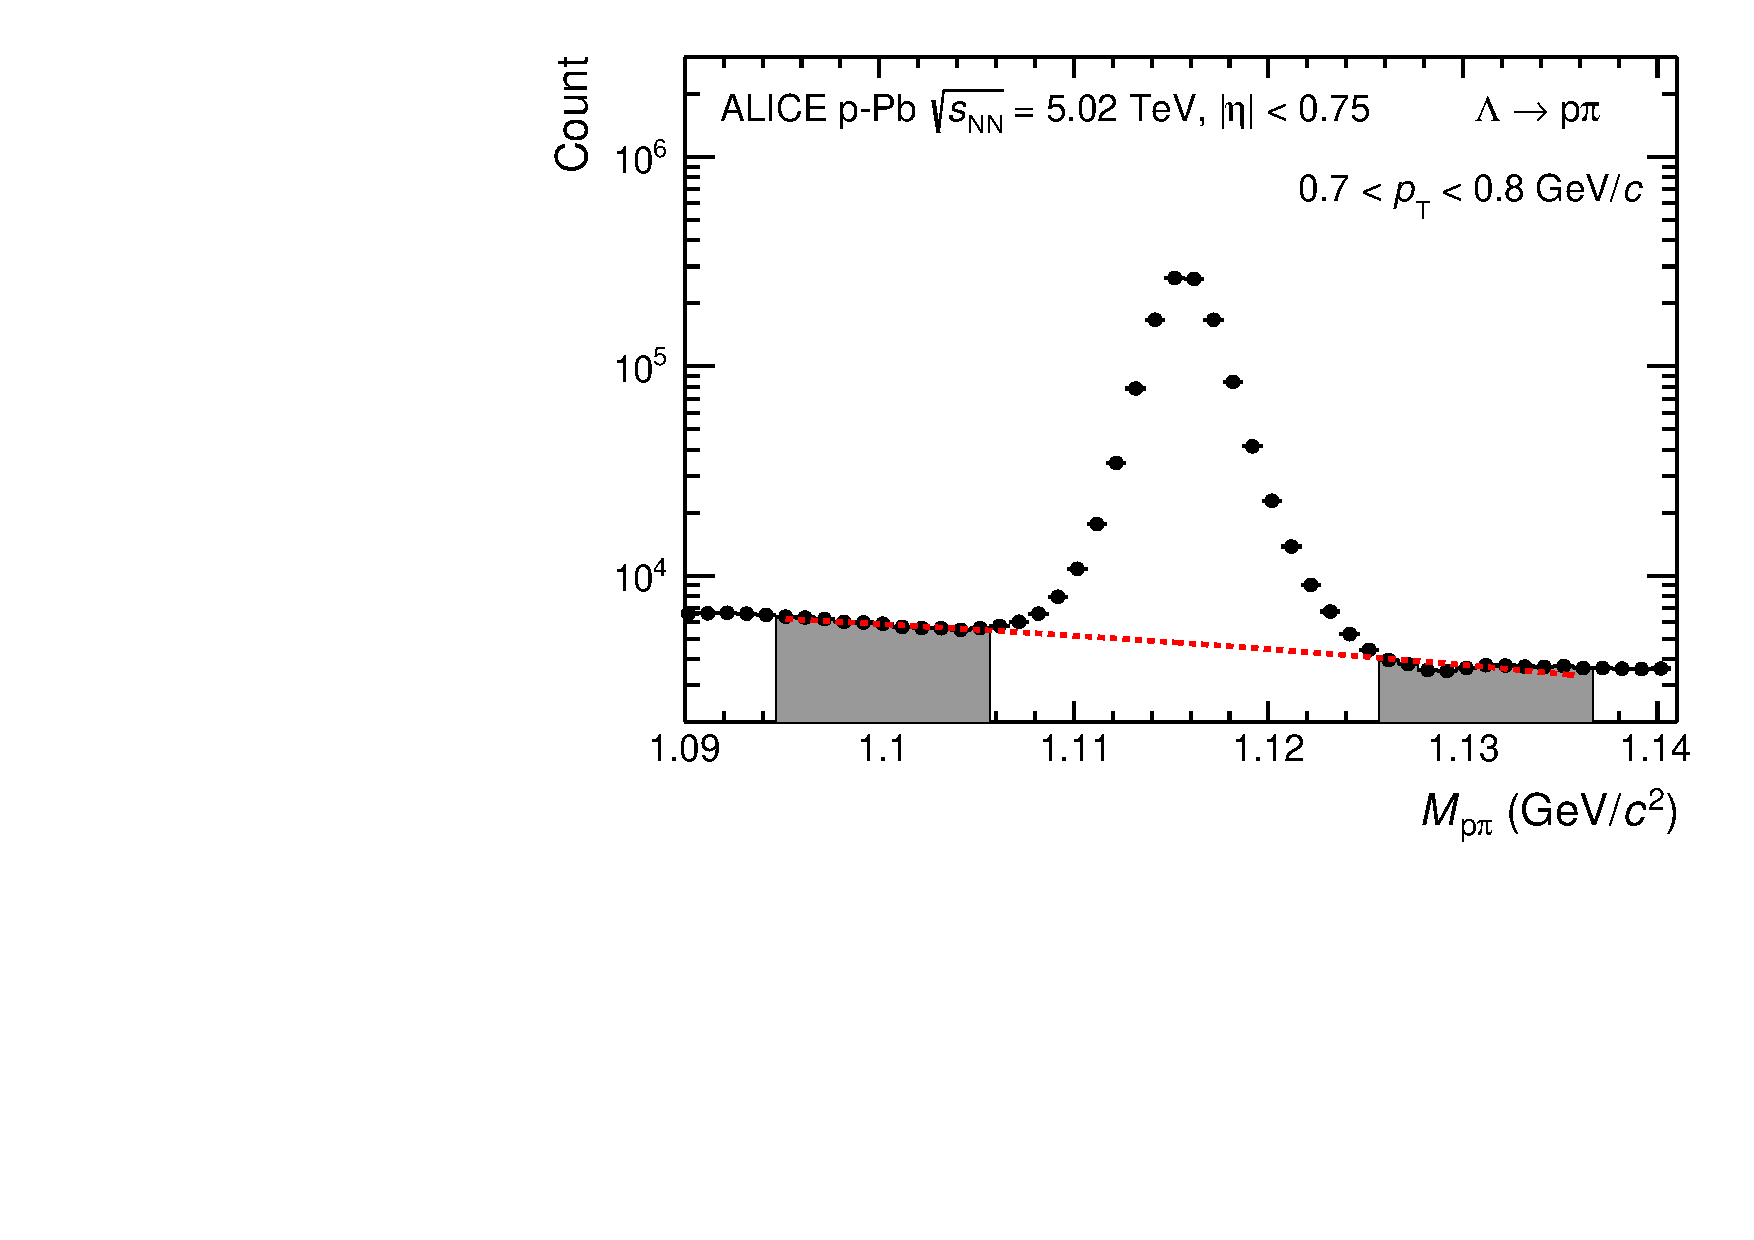
\includegraphics[width=.4\textwidth]{cf01_2}
		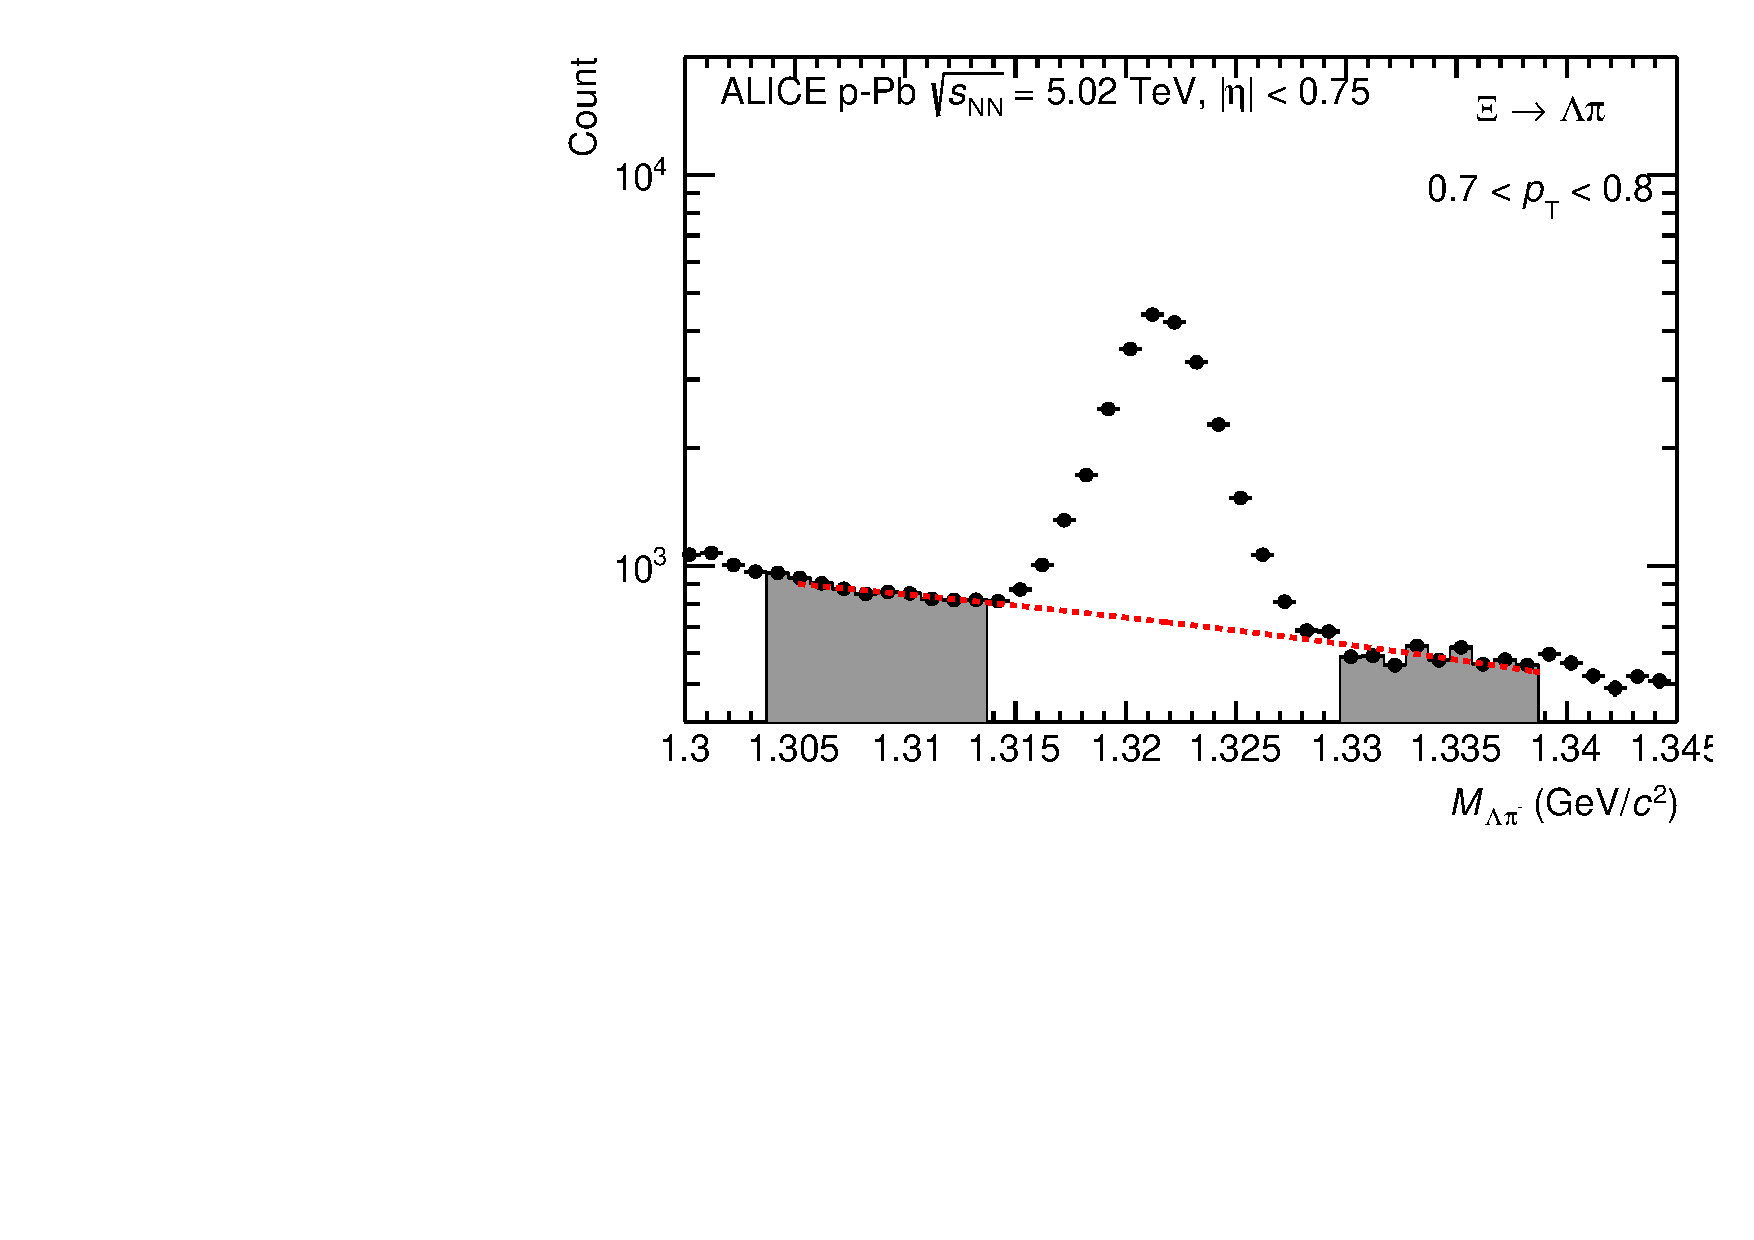
\includegraphics[width=.4\textwidth]{cf01_3}
		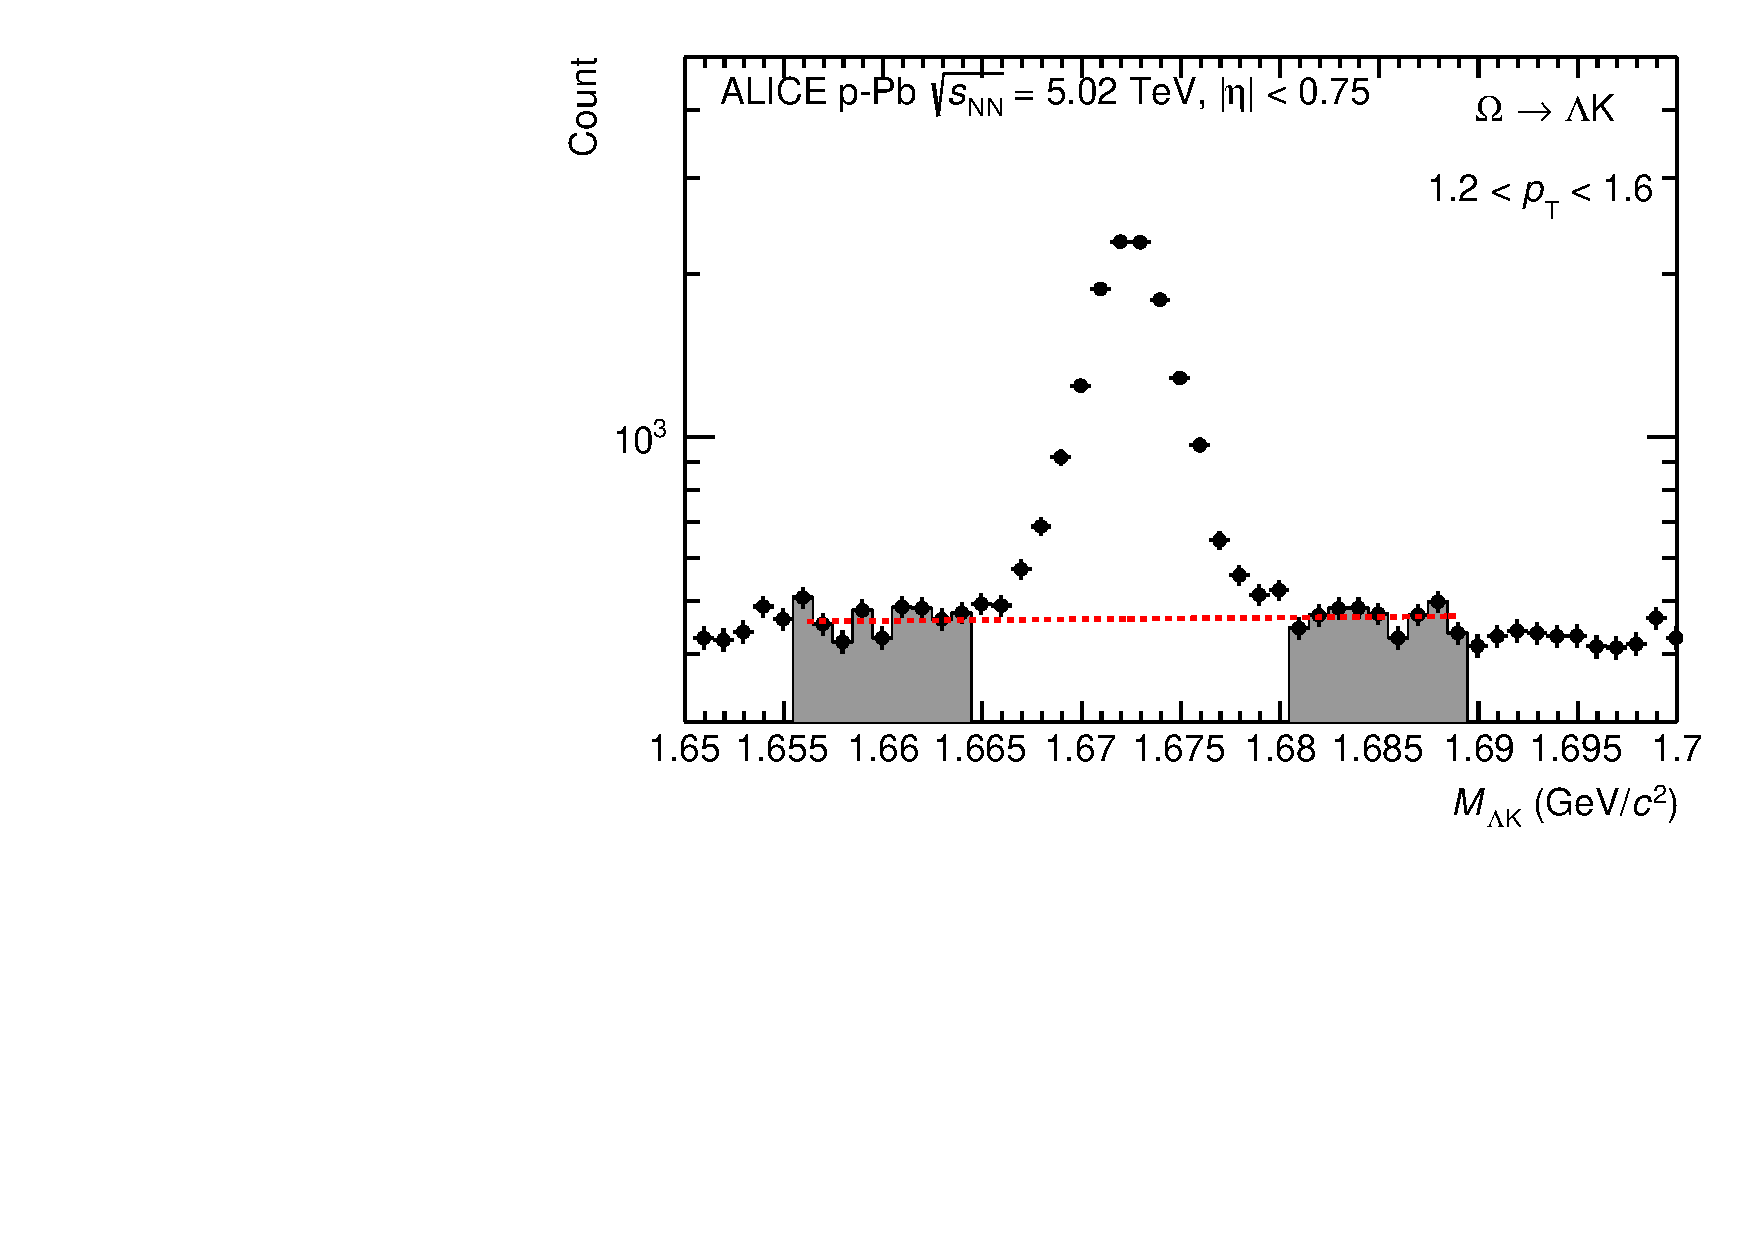
\includegraphics[width=.4\textwidth]{cf01_4}
		\caption{Invariant Mass distribution for $\kzero$, $\lmb$, $\Xi$ and $\Omega$ in different $\pT$ intervals in MB \pPb system. The candidates are reconstructed in $|\eta|<0.75$.
			The grey areas are used for signal extraction in the bin counting procedure.
			The red dashed lines represent the fit to the background distributions and the interpolate to the ``peak'' region.}
		\label{fig:InvM}
	\end{center}
\end{figure}

\subsection{Matching of strange particles to jets and underlying event}%
\label{sec:ParJetMatch}

The strategy of matching the (multi-)strange particles with jets follow those presented in earlier work~\cite{V0injet}.
The matching is done on a geometrical basis which presented in Eq.~\ref{eq:DParJet}.
\begin{equation}
d(\mathrm{particle, jet}) = \sqrt{(\eta_\mathrm{particle} -\eta_{\rm jet})^{2} + (\varphi_\mathrm{particle} -\varphi_{\rm jet})^{2}}
\label{eq:DParJet}
\end{equation}
If the distance between the particle candidate and the jet ($d$) is smaller than the matching distance $D$ (= 0.4), the candidate is considered to be inside the jet cone (JC).
The raw yields in JC are not only composed of the hadron produced via jet fragmentation (write as JE), but also hadron from Underlying Event (UE), which is defined as the sum of all particles which are not produced via hard parton fragmentation.
The UE contribution is estimated by Perpendicular Cone (PC) yields.
The PC indicates the cone, which is located in $\eta \times \varphi$ space in the perpendicular direction to the jet axis at the same $\eta$.
The systematic uncertainty due to the UE subtraction is estimated by the particle in Outside jet Cone(OC) yields.

In addiction, the acceptance selections of inclusive (regardless of the association between particle and hard scattering), JC and UE (multi-)strange particles are different in the $\eta$--$\varphi$ plane.
To get the particle from JE the production yields are normalized to per-acceptance density ($\rho$).
\begin{equation}
\begin{split}
{\rm Inclusive:}\qquad & \frac{\dd\rho}{\dd\pT} = \frac{1}{N_{\rm ev}}\times\frac{1}{\Delta\eta\Delta\varphi}\times\frac{\dd N}{\dd\pT} \\
{\rm JC:}\qquad & \frac{\dd\rho}{\dd\pT} = \frac{1}{N_{\rm ev}^{\rm jet}} \times\frac{1}{\mathcal{P}_{\rm JC}\Delta\eta\Delta\varphi}\times\frac{\dd N}{\dd\pT} \\
{\rm PC:}\qquad & \frac{\dd\rho}{\dd\pT} = \frac{1}{N_{\rm ev}^{\rm jet}} \times\frac{1}{\mathcal{P}_{\rm PC}\Delta\eta\Delta\varphi}\times\frac{\dd N}{\dd\pT} \\
{\rm OC:}\qquad & \frac{\dd\rho}{\dd\pT} = \frac{1}{N_{\rm ev}^{\rm jet}} \times\frac{1}{\mathcal{P}_{\rm OC}\Delta\eta\Delta\varphi}\times\frac{\dd N}{\dd\pT} \\
\end{split}
\label{eq:normalize}
\end{equation}
where the $\mathcal{P}$ denotes the probability of particles in a given selection found in the $\eta$--$\varphi$ plane with respect to the inclusive one.

\subsection{Corrections for strange particles reconstruction and feed-down}
\label{SubSec:Correction}
The reconstruction efficiency of particles are obtained in Monte Carlo simulated data.
These are estimated using PYTHIA 8.2~\cite{Sjostrand:2014zea} and DPMJet~\cite{Roesler:2000he} generators in \pp and \pPb, respectively, and tracsported through a GEANT 3~\cite{Brun:1994aa}.
Due to different $\eta$-shape between particle in JC and the inclusive one, it is needed to take the $\eta$ dependence of different particle distributions into account~\cite{V0injet}.
Fig.~\ref{fig:EffiJCIncl} shows the difference of reconstruction efficiency of JC particles and the inclusive one.
\begin{figure}[!ht]
	\begin{center}
		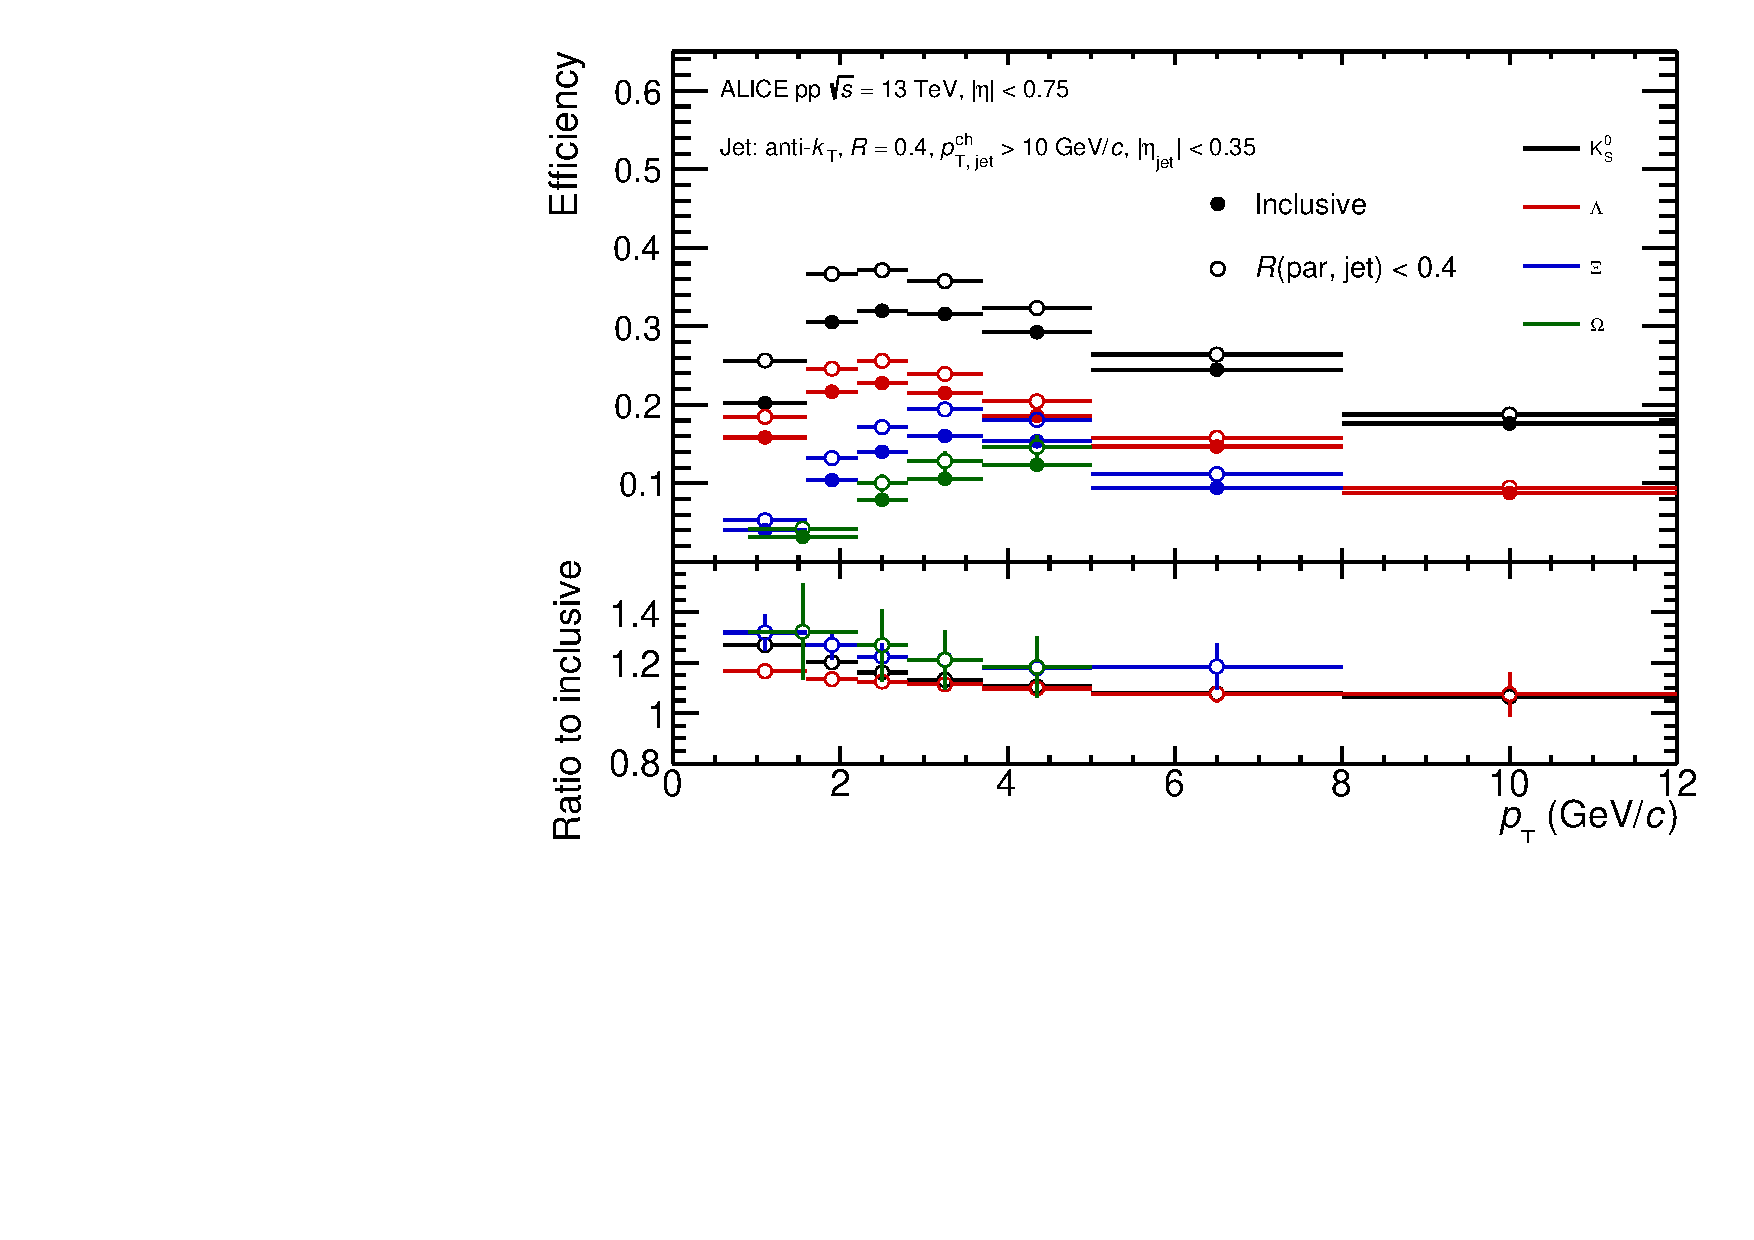
\includegraphics[width=.4\textwidth]{cf02_1}
		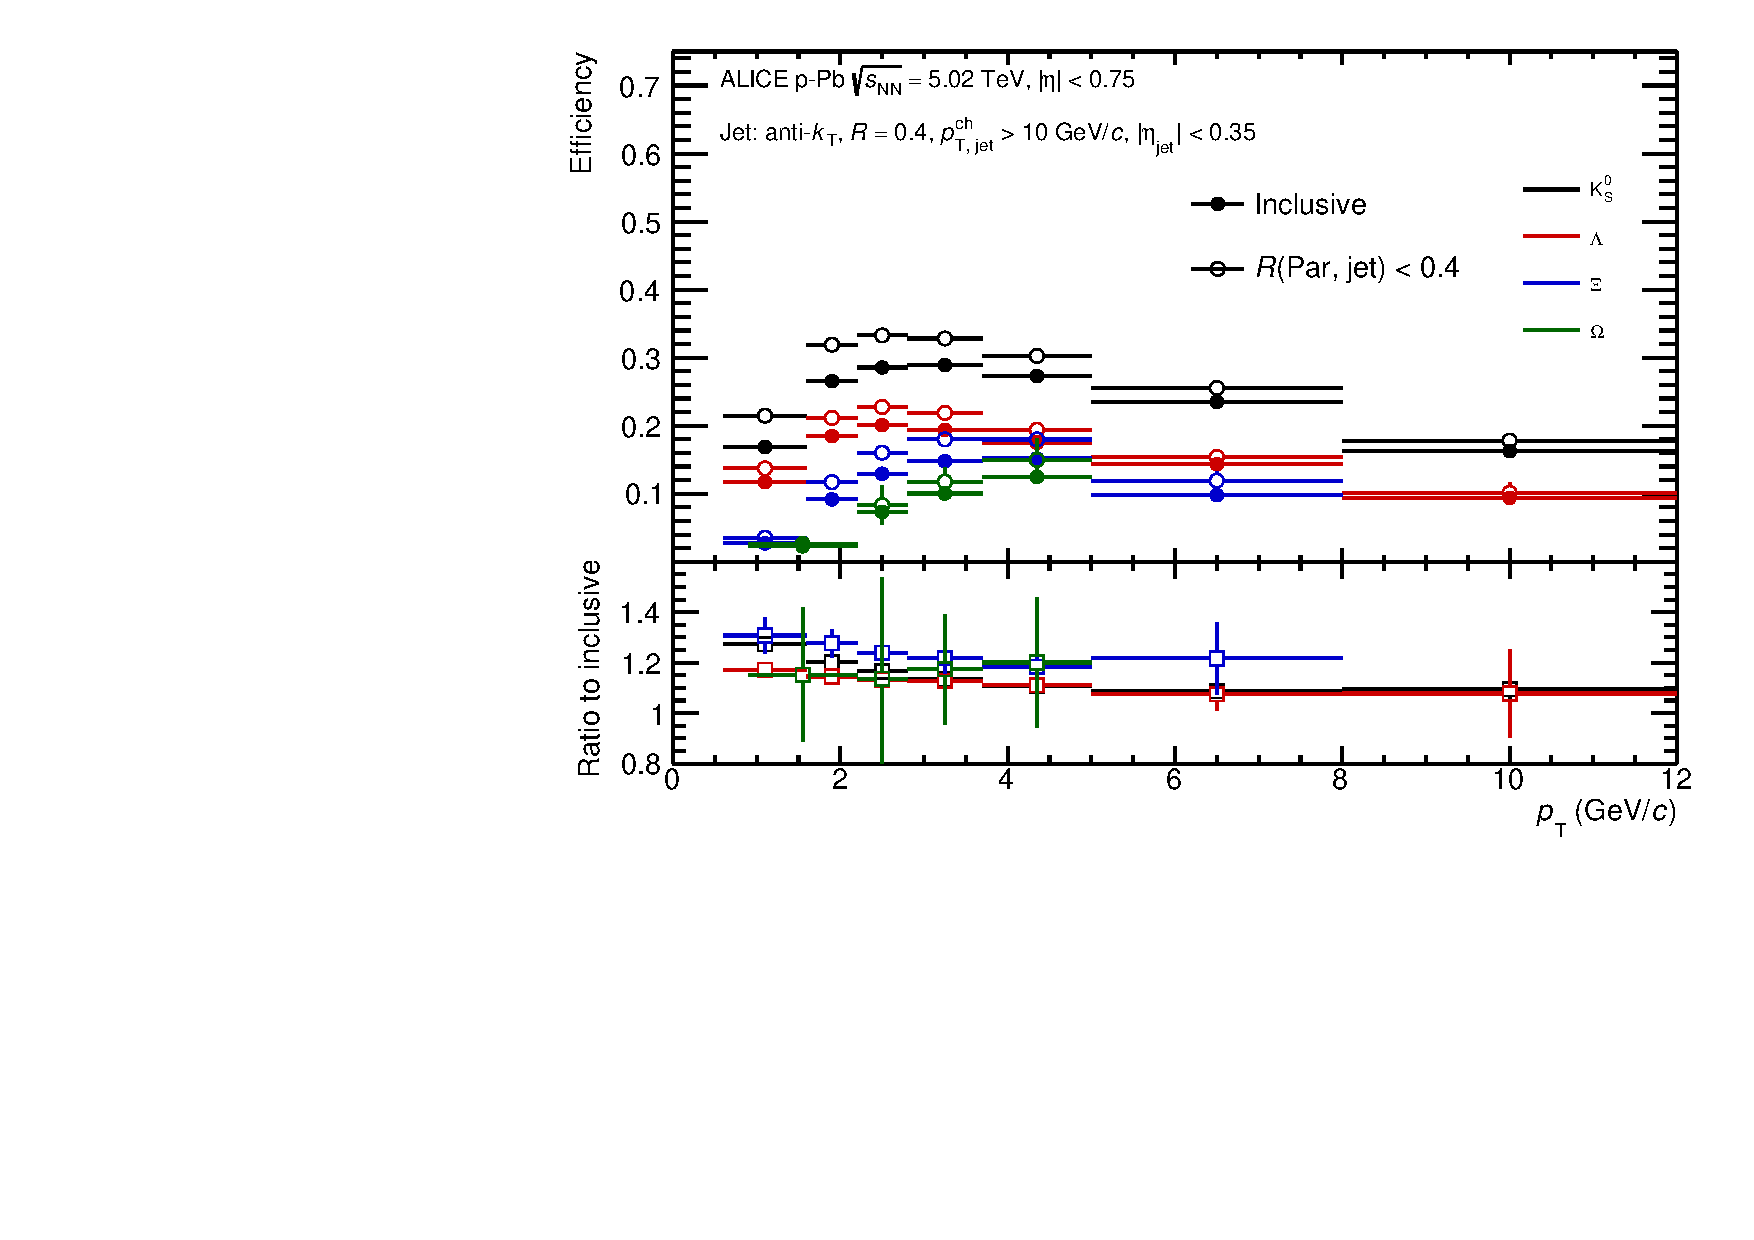
\includegraphics[width=.4\textwidth]{cf02_2}
	\end{center}
	\caption{The reconstruction efficiency for the particles in \pp collisions at \thirteen (left) and in \pPb collisions at \fivenn (right) for two selections: inside jet cone, $R(\mathrm{particle, jet}) < 0.4$ and the inclusive one.}
	\label{fig:EffiJCIncl}
\end{figure}

Only the yields for $\lmb$ and $\almb$ are significantly affected by secondary particles coming from the decays of charged and neutral $\Xi$ baryons.
The feed-down fraction is calculated with a data-driven approach~\cite{Abelev:2013haa}.
The detailed of inclusive feed-down method has been introduced in previous ALICE analysis works~\cite{Acharya:2019kyh, Acharya:2020uxl, ALICE:2017jyt}.
In particular, the $\lmb$ and $\almb$ in jet and UE feed-down component usually estimated by inclusive $\Xis$ spectra and PYTHIA simulations~\cite{V0injet}, due to lack of $\Xis$ in jet and UE results.
In this work, the feed-down fraction in jets and UE is computed for each $\pT$ bin by the measured $\Xis$ in jets and UE spectra, thereby assuming that the production rates of charged and neutral $\Xi$ are equal.
Figure~\ref{fig:FdFrac} shows the results of feed-down fraction in JC and the inclusive one.
\begin{figure}[!ht]
	\begin{center}
		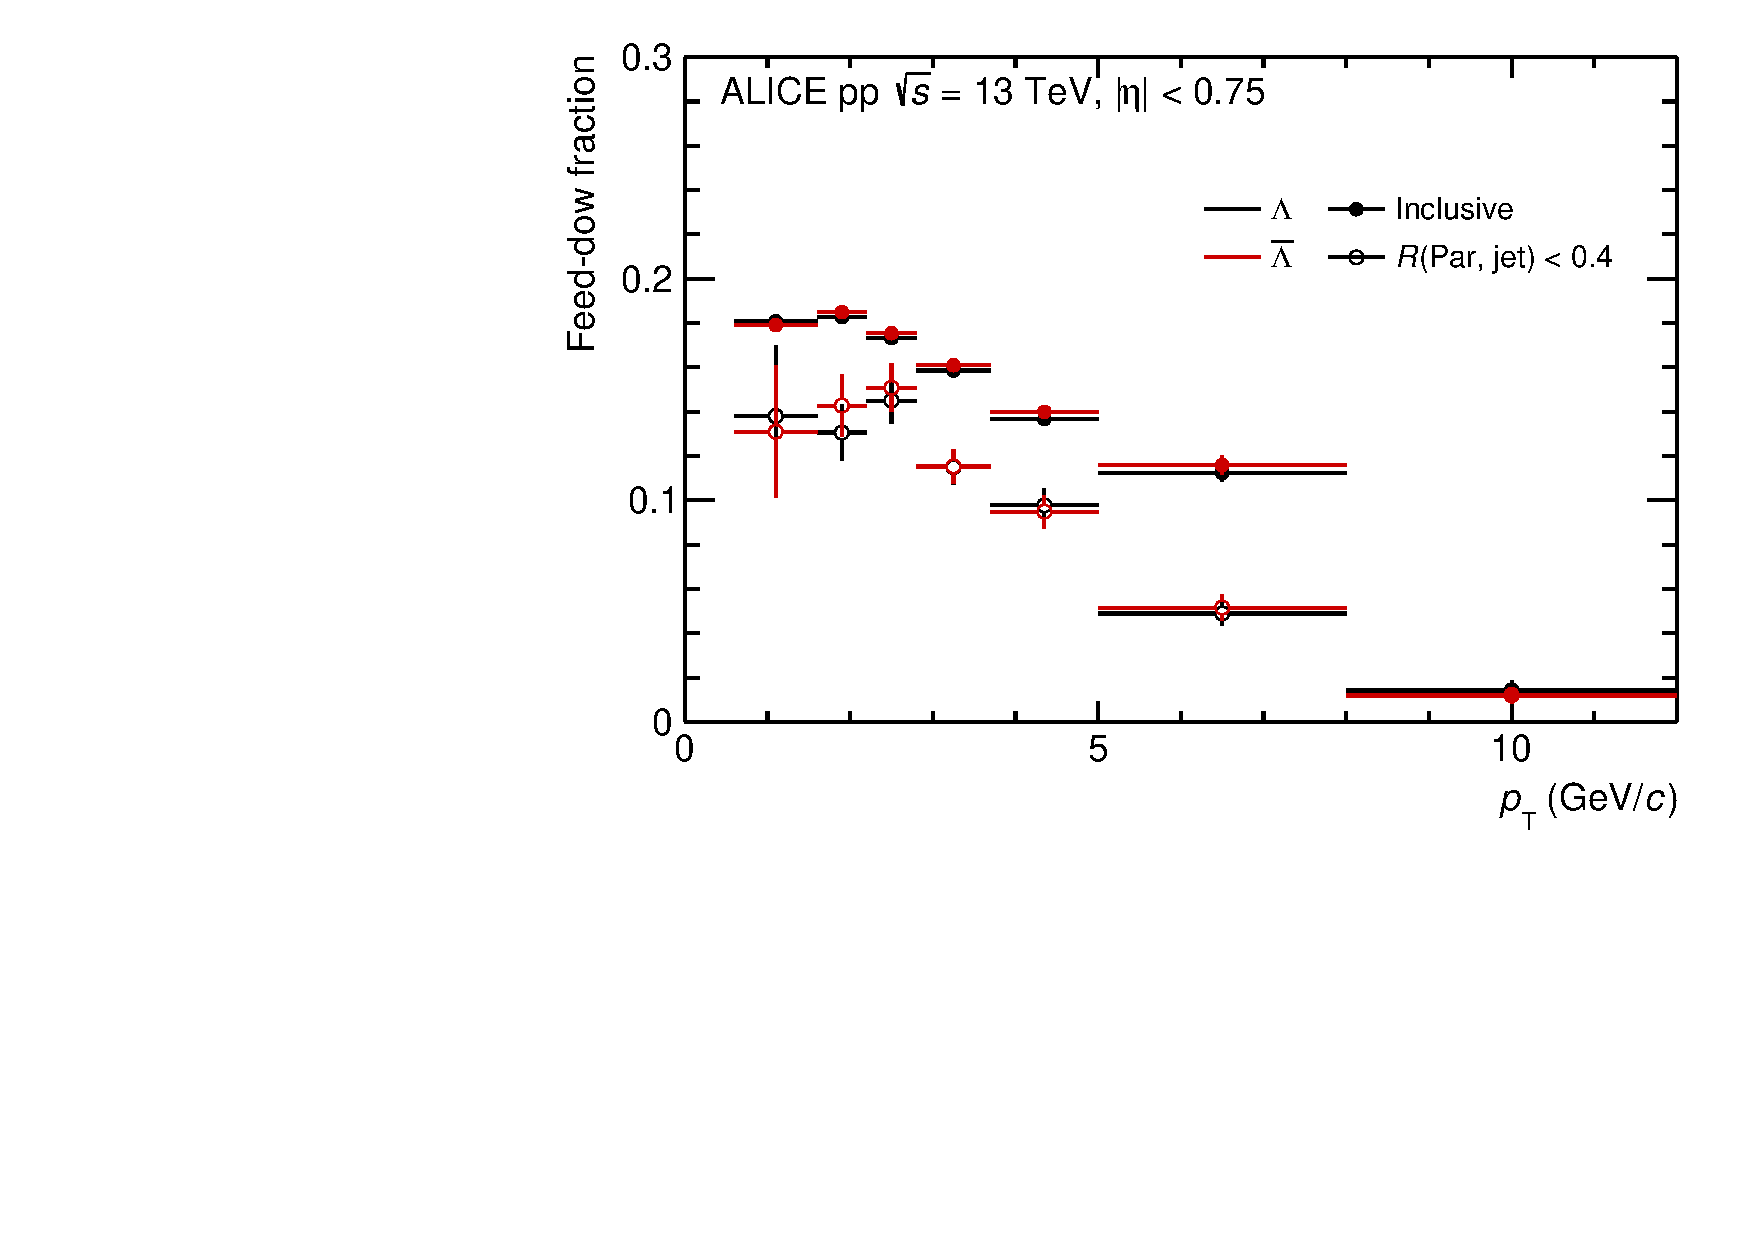
\includegraphics[width=.4\textwidth]{cf03_1}
		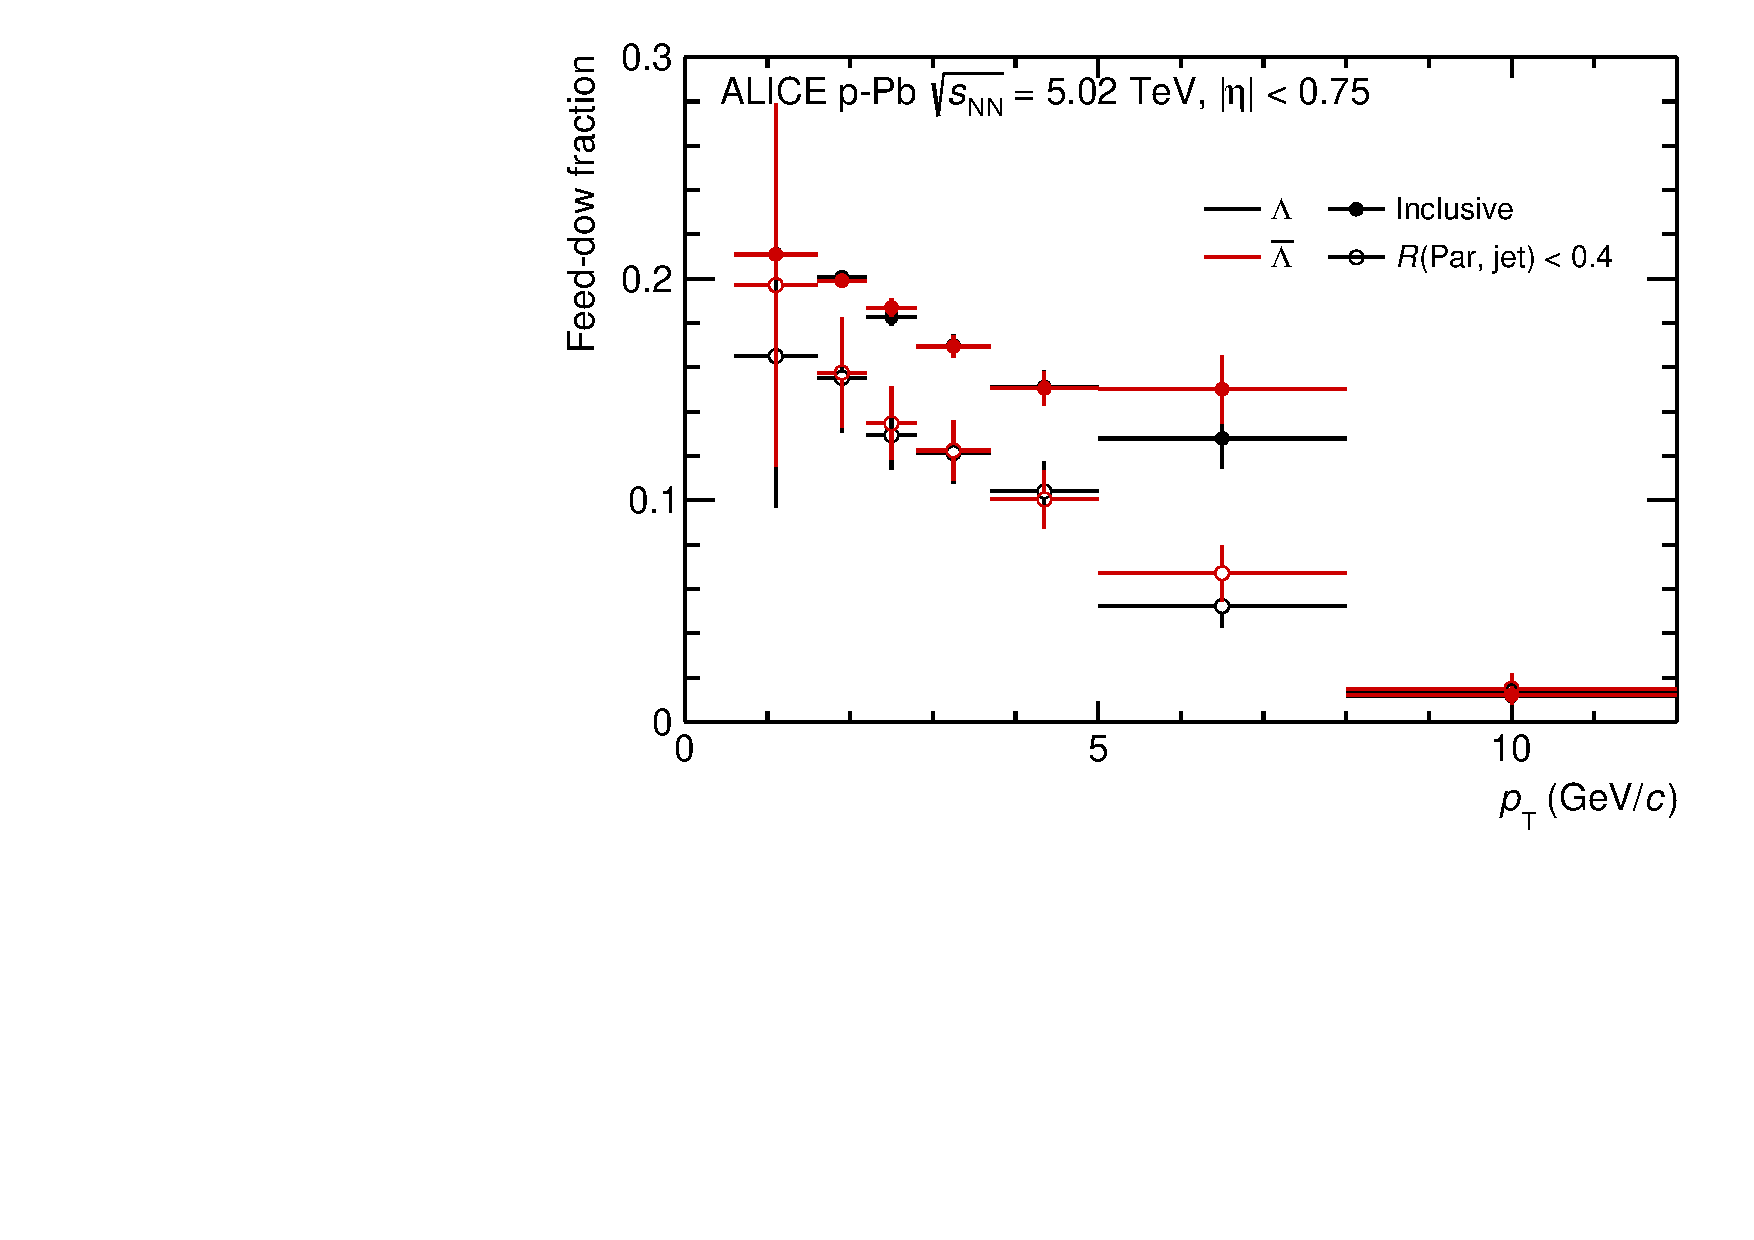
\includegraphics[width=.4\textwidth]{cf03_2}
	\end{center}
	\caption{Fraction of $\lmb$ spectra removed due to feed-down subtraction of charged and neutral $\Xi$}
	\label{fig:FdFrac}
\end{figure}

\subsection{Systematic uncertainties}
\label{sec:SysUncer}
The total systematic uncertainty, for $\kzero$, $\lmb$, $\almb$, $\Xis$ and $\Oms$ reconstruction of each data point of the final results, due to the choice of selection criteria are estimated separately in each $\pT$ interval.
Individual settings are loosened and tightened, in order to measure changes in the signal loss correction.
The main sources of the systematic uncertainty in this measurements are knowledge of detector materials, track selections, particle identification, proper lifetime, topological selection and signal extraction.
All these individual error contributions, which are listed in Tab.~\ref{tab:ppInclUncer}, \ref{tab:pPbInclUncer} are added in quadrature.
\begin{table}[!ht]
	\begin{center}
		\caption{Main sources and values of the relative systematic uncertainties(\%) of $\kzero$, $\lmb + \almb$, $\X + \Ix$ and $\Om + \Mo$ in \pp collisions at \thirteen.
			The value are reported for low, intermediate and high $\pT$.}
		\label{tab:ppInclUncer}
		\begin{tabularx}{\textwidth}{@{} lCCCCCCCCCCCC @{}}
			\toprule
			\textbf{Uncertainty source} & \multicolumn{3}{c}{\textbf{$\kzero$}}
			& \multicolumn{3}{c}{\textbf{$\lmb + \almb$}}
			& \multicolumn{3}{c}{\textbf{$\X + \Ix$}}
			& \multicolumn{3}{c}{\textbf{$\Om + \Mo$}} \\
			\cmidrule(lr){2-4} \cmidrule(lr){5-7} \cmidrule(lr){8-10} \cmidrule(lr){11-13}
			$\pT$ (\GeVc)    & 0.6 & 2 &10  & 0.6 & 2 & 10  & 0.6 & 2 & 7   & 0.6& 2 & 5 \\
			\midrule
			Detector material & 4 & 4 & 4 & 4 & 4 & 4 & 4 & 4 & 4 & 4 & 4 & 4 \\
			Track selection &  & 0.4 & 0.4 & 0.4 & 0.4 & 0.4 & 0.4 & 0.4 & 0.4 & 0.4 & 0.4 & 0.4\\
			Particle identification \\
			Proper lifetime \\
			Topological \\
			Signal extraction \\
			\midrule
			\textbf{Total uncertainty}\\
			\bottomrule
		\end{tabularx}
	\end{center}
\end{table}

\begin{table}[!ht]
	\begin{center}
		\caption{Main sources and values of the relative systematic uncertainties(\%) of $\kzero$, $\lmb + \almb$, $\X + \Ix$ and $\Om + \Mo$ in \pPb collisions at \fivenn.
			The value are reported for low, intermediate and high $\pT$.}
		\label{tab:pPbInclUncer}
		\begin{tabularx}{\textwidth}{@{} lCCCCCCCCCCCC @{}}
			\toprule
			\textbf{Uncertainty source} & \multicolumn{3}{c}{\textbf{\kzero}}
			& \multicolumn{3}{c}{\textbf{$\lmb + \almb$}}
			& \multicolumn{3}{c}{\textbf{$\X + \Ix$}}
			& \multicolumn{3}{c}{\textbf{$\Om + \Mo$}} \\
			\cmidrule(lr){2-4} \cmidrule(lr){5-7} \cmidrule(lr){8-10} \cmidrule(lr){11-13}
			$\pT$ (\GeVc) & 0.6 & 2 &10  & 0.6 & 2 & 10    & 0.6 & 2 & 7   & 0.6& 2 & 5 \\
			\midrule
			Detector material& 0.4 & 0.4 & 0.4 & 0.4 & 0.4 & 0.4 & 0.4 & 0.4 & 0.4 & 0.4 & 0.4 & 0.4 \\
			Track selection \\
			Particle identification \\
			Proper lifetime \\
			Topological \\
			Signal extraction\\
			\midrule
			\textbf{Total uncertainty} \\
			\bottomrule
		\end{tabularx}
	\end{center}
\end{table}

\textbf{Material budget.} The effect of the incomplete knowledge of the detector's material budget is evaluated by comparing different Monte Carlo simulations in which the material budget was increased and decreased by $4.5\%$.
This value corresponds to the uncertainty on the determination of the material budget by measuring photon conversions.
This particular systematic uncertainty is around $0.4\%$.

\textbf{Track selection.} To estimate the systematic due to the track selection, the analysis has been redone with the increased number of required clusters in the TPC.

\textbf{Particle identification.} The TPC $\dEdx$ selection is used to reduce the combinatorial background in the (multi-)strange particle invariant mass distribution.
The number of $\sigma$ in the identification of particles using the $\dEdx$ have been varied between $4\sigma$ to $6\sigma$.

\textbf{Proper lifetime selection.} The proper lifetime defied as $mLc/p$, which $m$ is the mass of particles, $L$ is the decay length, and $p$ is the particle's momentum.
The selection on the $mLc/p$ is varied from around $12$ to $40$~cm for $\kzero$, $20$ to $40$ cm for $\lmb$ $(\almb)$ and $2c\tau$ to $6c\tau$ for $\Xis$ and $\Oms$.

\textbf{Topological selection.} The values of the selection criteria on the topological variables are varied around their nominal values.
The observed deviations for each component are summed in quadrature.

\textbf{Signal extraction.} In the same spirit, the signal extraction technique has been tested by varying the widths used to define the ``signal" and ``background'' regions, expressed in terms of the number of $\sigma$ as defined in Sec.~\ref{sec:ParRec}.

The additional systematic uncertainty sources associated with particle yield in jet are originated from the UE subtraction estimator and the jet $\pT$ threshold.
In Sec.~\ref{sec:ParJetMatch}, it introduced two UE estimators, the PC and OC.
From the deviation of OC and PC, the relative systematic uncertainty of the UE subtraction is obtained.
To estimate the effect of jet $\pT$ thresholds uncertainty, the analysis is repeated with the jet $\pT$ cut $10\pm 1$~\GeVc.
The systematic of the particle in jets are added to the list of uncertainties in quadrature.
The value are shown in Table~\ref{tab:ppJEUncer}, \ref{tab:pPbJEUncer}.

\begin{table}[!ht]
	\begin{center}
		\caption{Main sources and values of the relative systematic uncertainties(\%) of $\kzero$, $\lmb + \almb$, $\X + \Ix$ and $\Om + \Mo$ in JE in \pp collisions at \thirteen.
			The value are reported for low, intermediate and high $\pT$.}
		\label{tab:ppJEUncer}
		\begin{tabularx}{\textwidth}{@{} lCCCCCCCCCCCC @{}}
			\toprule
			\textbf{Uncertainty source} & \multicolumn{3}{c}{\textbf{\kzero}}
			& \multicolumn{3}{c}{\textbf{$\lmb + \almb$}}
			& \multicolumn{3}{c}{\textbf{$\X + \Ix$}}
			& \multicolumn{3}{c}{\textbf{$\Om + \Mo$}} \\
			\cmidrule(lr){2-4} \cmidrule(lr){5-7} \cmidrule(lr){8-10} \cmidrule(lr){11-13}
			$\pT$ (\GeVc) & 0.6 & 2 &10  & 0.6 & 2 & 10    & 0.6 & 2 & 7   & 0.6& 2 & 5 \\
			\midrule
			Particle reconstruction\\
			UE subtraction\\
			Jet $\pT$ threshold\\
			\midrule
			\textbf{Total uncertainty} \\
			\bottomrule
		\end{tabularx}
	\end{center}
\end{table}

\begin{table}[!ht]
	\begin{center}
		\caption{Main sources and values of the relative systematic uncertainties(\%) of $\kzero$, $\lmb + \almb$, $\X + \Ix$ and $\Om + \Mo$ in JE in \pPb collisions at \fivenn.
			The value are reported for low, intermediate and high $\pT$.}
		\label{tab:pPbJEUncer}
		\begin{tabularx}{\textwidth}{@{} lCCCCCCCCCCCC @{}}
			\toprule
			\textbf{Uncertainty source} & \multicolumn{3}{c}{\textbf{\kzero}}
			& \multicolumn{3}{c}{\textbf{$\lmb + \almb$}}
			& \multicolumn{3}{c}{\textbf{$\X + \Ix$}}
			& \multicolumn{3}{c}{\textbf{$\Om + \Mo$}} \\
			\cmidrule(lr){2-4} \cmidrule(lr){5-7} \cmidrule(lr){8-10} \cmidrule(lr){11-13}
			$\pT$ (\GeVc) & 0.6 & 2 &10  & 0.6 & 2 & 10    & 0.6 & 2 & 7   & 0.6& 2 & 5 \\
			\midrule
			Particle reconstruction\\
			UE subtraction\\
			Jet $\pT$ threshold\\
			\midrule
			\textbf{Total uncertainty} \\
			\bottomrule
		\end{tabularx}
	\end{center}
\end{table}

The uncertainty of jet cone particle ratios ($\lmb/\kzero$, $\Xi/\kzero$, $\Omega/\kzero$, $\Xi/\lmb$, $\Omega/\lmb$ and $\Omega/\Xi$) also consider three sources: the particle reconstruction, UE subtraction and the jet $\pT$ threshold.
The particle reconstruction uncertainty is propagated from the spectra.
Uncertainties related to UE subtraction and jet $\pT$ threshold are obtained by varying the condition in both numerator and denominator of the corresponding ratios.
\emp{update uncertainty values later}

%\begin{table}[!ht]
%	\begin{center}
%		\caption{Main sources and values of the relative systematic uncertainties(\%) of $\lmb/\kzero$, $\Xi/\kzero$, $\Omega/\kzero$, $\Xi/\lmb$, $\Omega/\lmb$ and $\Omega/\Xi$ in JE in \pp collisions at \thirteen.
%			The value are reported for low, intermediate and high $\pT$.}
%		\label{tab:ppRatioUncer}
%		\begin{tabularx}{\textwidth}{@{} lCCCCCC @{}}
%			\toprule
%			\textbf{Uncertainty source} & \textbf{$\frac{\lmb + \almb}{2\kzero}$} & \textbf{$\frac{\X + \Ix}{2\kzero}$} & \textbf{$\frac{\Om + \Mo}{2\kzero}$} & \textbf{$\frac{\X + \Ix}{\lmb + \almb}$} & \textbf{$\frac{\Om + \Mo}{\lmb + \almb}$} & \textbf{$\frac{\Om + \Mo}{\X + \Ix}$}\\
%			$\pT$ (\GeVc) & [0.6 -2 -10]   & [0.6 -2 -10] & [0.6 -2 -10] & [0.6 -2 -10]  & [0.6 -2 -10] & [0.6 -2 -10]\\
%			\midrule
%			Particle reconstruction\\
%			UE subtraction\\
%			Jet $\pT$ threshold\\
%			\midrule
%			\textbf{Total uncertainty} \\
%			\bottomrule
%		\end{tabularx}
%	\end{center}
%\end{table}
